\documentclass[a4j,10pt]{jsarticle}
\usepackage{listings, jlisting}
\usepackage{mylatex}
\usepackage{ap3}
\usepackage{ascmac}
\usepackage[dvipdfmx]{graphicx}
\usepackage{here}

% プリアンブル
\title{タイトル}
\author{著者名1 \and 著者名2}
\date{2009/05/24 \\ \today}

\begin{document}
  % タイトルを出力
  \maketitle

  % 目次の表示
  \tableofcontents
  \newpage

  \section{タイトル}

  \subsection{タイトルの出力例}

  \begin{table}[H]
    \caption{値段表}
    \centering
    \begin{tabular}{|l|l|} \hline
      コマンド & 解説 \\ \hline \hline
      \textbackslash title & タイトル (文書名) \\ \hline
      \textbackslash author & 著者名 (著者が複数いる場合は \textbackslash and コマンドで区切る) \\ \hline
      \textbackslash date & 日付 \\ \hline
      \textbackslash maketitle & 上記で指定されたタイトルの出力 \\ \hline
    \end{tabular}
  \end{table}

  \begin{lstlisting}[label=titlesample1, caption=LaTeXサンプル, language=TeX]
    \documentclass[11pt,a4j]{jarticle}

    % プリアンブル
    \title{タイトル}
    \author{著者名1 \and 著者名2}
    \date{2009/05/24}
    
    \begin{document}
      % タイトルを出力
      \maketitle
    
      \section{節}
      文章
    \end{document}
  \end{lstlisting}
  
  \begin{figure}[H]
    \centering
      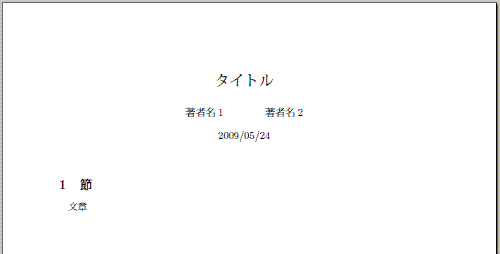
\includegraphics[height=60mm]{src/title.jpg}
    \caption{LaTeXサンプル実行結果}
    \label{fig:titlesample1}
   \end{figure}


  \begin{thebibliography}{9}
    \bibitem{reference_site} Latexコマンド集 - (http://www.latex-cmd.com/) 
  \end{thebibliography}

\end{document}

\end{document}

